\section{Introduction}
Modern laser and trapping techniques allow us to study a wide range phenomena with ultra-cold atoms. Traditionally, a fixed potential by a laser was being used, e.g. tow opposing laser beams. However, with such a setup several areas of condensed matter research (such as supersolidity, etc.) remain inaccessible due to the rigid nature of the laser potential. If we, however, place the atoms in a cavity, they will interact with the cavity mode and self-induce a potential, thus enabling us to study a wider range of phenomena. Consider a Bose-Einstein Condensate (BEC) in a cavity interacting with the cavity mode and a pump laser. Atoms coherently scatter light of the laser, those separated by $\lambda_\text{cav}$ emit in phase and populate the cavity with photons, leading to enhancement of atom-cavity coupling. If the laser is far red-detuned, the atoms will couple more strongly to the cavity, trapping them at even or odd antinodes which leads to even more superradience and stronger coupling. A steady state is reached when the energetic gain from superradience is balanced by the kinetic energy of repulsion.


\section{Optical cavities}
There are different types of cavities, such as the bow-tie, the ring and the Fabry-Perot cavity. In the case of the Fabry-Perot cavity, there are two curved mirrors separated by a distance $d$. If $d = n \lambda / 2$, the system is in resonance and there's a strong light field in the cavity. Thus boundary conditions on light space determine the modes of the frequency space. An illustration of a Fabry-Perot cavity with longitudinal and transversal pumping can be seen in Figure~\ref{pumping}.

\begin{figure}[!htb]
	\begin{minipage}[b]{.5\linewidth}
	\centering
	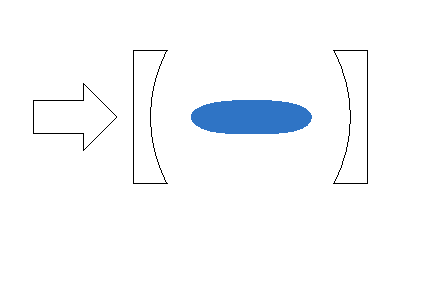
\includegraphics[width=.8\linewidth]{images/pump_long.eps}
	\subcaption{Longitudinal pumping.}
	\end{minipage}
%
	\begin{minipage}[b]{.5\linewidth}
	\centering
	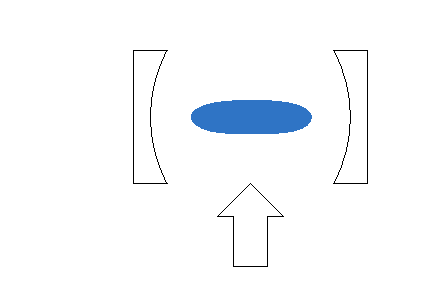
\includegraphics[width=.8\linewidth]{images/pump_trans.eps}
	\subcaption{Transversal pumping.}
	\end{minipage}
\caption{Longitudinal and transversal pumping.}
\label{pumping}
\end{figure}
\FloatBarrier

\section{Derivation of the Hamiltonian}
For those wishing to refresh their knowledge of quantum mechanics, the introductory chapters of Fox's quantum optics book will be a great help \cite{fox}. In this section we'll derive the Hamiltonians being used for the simulation; one Hamiltonian for longitudinal pumping and one for transversal pumping. The Hamilton operator represents the total energy of a quantum system. We'll start with the Jaynes-Cummings Hamiltonian which describes the interaction of a two-level atom with a single mode of a cavity-field. We'll then modify the Hamiltonian according to our needs step by step. We'll tackle the crucial details and reference parts of the derivation which is not presented here.

\subsection{The Jaynes-Cummings Hamiltonian}
The Jaynes-Cummings model describes the interaction of a two-level atom with a single mode of a cavity field. The first appearance was in \cite{jaynes}. We'll restrict ourselves to one dimension and start with an atom (or a BEC) in an external potential:

\begin{align}
H_0 = \frac{p^2}{2m} + V_\text{ext}(x).
\end{align}Now we place that atom in a cavity and it will interact with the cavity mode, creating more terms in our Hamiltonian that we have to consider. First, there's the energy of the field:

\begin{align}
H_\text{field} = -\hbar \omega_\text{c} a^\dagger a,
\end{align}where $\omega_\text{c}$ is the resonance frequency of the cavity and $a^\dagger$ and $a$ are the creation and annihilation operators. Next, we'll add a term describing the atomic transitions:

\begin{align}
H_\text{transition} = -\frac{1}{2}\hbar \omega_\text{a} \sigma_z,
\end{align}where $\omega_\text{a}$ is the resonance frequency of the atom and $\sigma_z$ is the Pauli z-matrix. The above term describes the atom being in the ground state or excited state, the transition energy is $1/2\hbar \omega_\text{a}$. The field-atom interaction we describe with following term:

\begin{align}
H_\text{interaction} = \hbar g_0 \cos(kx) (\sigma^+ a + \sigma^- a^\dagger),
\end{align}where $g_0$ is the coupling strength and $\sigma^+$ and $\sigma^-$ are the raising and lowering operators. Finally, we'll add the term describing the pumping:

\begin{align}
H_\text{pump} = \hbar \eta (a e^{i\omega_\text{l}t} + a^\dagger e^{-i\omega_\text{l}t}),
\end{align}where $\eta$ is the pumping strength and $\omega_\text{l}$ is the laser frequency. We now have the full Jaynes-Cummings Hamiltonian which is the sum of all terms above:

\begin{align}
\begin{split}
H_\text{JC} = \underbrace{p^2 / 2m}_\text{atom} + \underbrace{V_\text{ext}(x)}_\text{external potential} - \underbrace{1/2 \hbar \omega_\text{a} \sigma_z}_\text{atomic transitions} - \underbrace{\hbar \omega_\text{c} a^\dagger a}_\text{field} + \underbrace{\hbar \eta (a e^{i \omega_\text{l} t} + a^\dagger e^{-i \omega_\text{l} t})}_\text{pumping} + \\
+ \underbrace{\hbar g_0 \cos(kx) (\sigma^+ a + \sigma^- a^\dagger)}_\text{field-atom interaction}.
\end{split}
\end{align}A more detailed derivation of the Jaynes-Cummings Hamiltonian (starting from Maxwell's equations and quantizing the cavity mode) can be found at \cite{collapseandrevival}. In order to get rid of the explicit time-dependence, we transform the Hamiltonian to a frame rotating with $\omega_\text{l}$. The Hamiltonian now reads:

\begin{align}
\begin{split}
H_\text{JC} = \frac{p^2}{2m} + V_\text{ext}(x) - \hbar \Delta_\text{a} \sigma_z - \hbar \Delta_\text{c} a^\dagger a + \hbar \eta (a + a^\dagger) + \\
+ \hbar g_0 \cos(kx) (\sigma^+ a + \sigma^- a^\dagger),
\end{split}
\end{align}where $\Delta_\text{a} = \omega_\text{l} - \omega_\text{a}$ and $\Delta_\text{c} = \omega_\text{l} - \omega_\text{c}$.

\subsection{Detuning}
The derivation for the Hamiltonians for the following sections is taken from \cite{donner}. In our case, the pumping laser is far detuned from the atomic resonance frequency, i.e. $\Delta_\text{a} = \omega_\text{l} - \omega_\text{a}$ is large. Thus the excitation probability of the atom is vanishing and we approximate $\sigma_z \approx 1/2$ because the atom stays mostly in the ground state. Now we derive heuristically a modified Hamiltonian. Going to the Heisenberg picture, we get:

\begin{align}
\dot{a} = \frac{i}{\hbar} [H, a] = i \Delta_\text{c} a - i \eta -i g_0 \cos(kx) \sigma^-.
\label{a_dot}
\end{align}Obviously, the kinetic energy and potential term vanish under the commutator. For the other terms:

\begin{align}
a^\dagger a = N \qquad [N, a] = -a \\
(a + a^\dagger) a - a (a + a^\dagger) = aa + a^\dagger a - aa - aa^\dagger & = 1 \\
\text{because we know:} \quad aa^\dagger & = a^\dagger a + 1 \nonumber \\
?? \quad \text{idk, check with instructor}
\end{align}A good reference for the commutator relation is \cite{bertlmann}. The time-derivative for the raising operator reads:

\begin{align}
\dot{\sigma}^+ = -i \Delta_\text{a} \sigma^+ + i g_0 \cos(kx) a^\dagger.
\end{align}We're not interested in fast dynamics, so we set $\dot{\sigma}^+ = 0$. We obtain

\begin{align}
\sigma^+ = \frac{g_0 }{\Delta_\text{a}} \cos(kx) a^\dagger && \sigma^- = \frac{g_0 }{\Delta_\text{a}} \cos(kx) a.
\end{align}Putting the above relation in equation~\ref{a_dot}, we get:

\begin{align}
\dot{a} = -i \Delta_\text{c} a + \frac{i g_0}{\Delta_\text{a}}  \cos(kx) a - i \eta.
\end{align}We can thus make a guess of the effective Hamiltonian:

\begin{align}
H_\text{long} = \frac{p^2}{2m} = V_\text{ext}(x) - \hbar \Delta_\text{c} a^\dagger a + \hbar \eta (a + a^\dagger) + \hbar U_0 \cos(kx)^2,
\end{align}where we set $U_0 \coloneqq g_0^2 / \Delta_\text{a}$. Note that because $H_\text{long} \propto \cos(kx)^2$, the Hamiltonian is $\lambda / 2$-periodic. Later in the simulation program, we want to make sure all quantities are expressed with the recoil energy $E_r = \hbar \omega_r$, where $\omega_r = \hbar k^2 / 2m$ is the recoil frequency. Therefore we factor our $E_r$ to see what we have to type into the program:

\begin{align}
\begin{split}
H_\text{long} = \hbar \omega_r \biggl( \frac{1}{\hbar^2 k^2} p^2 + \frac{1}{\hbar \omega_r} V_\text{ext}(x) - \frac{1}{\omega_r} \Delta_c a^\dagger a + \frac{1}{\omega_r} \eta (a + a^\dagger) + \\
 + \frac{1}{\hbar \omega_r} U_0 \cos(kx)^2 a^\dagger a \biggr).
\end{split}
\end{align}In the simulation program, we will thus set $\hbar = 1$ and multiply each quantity by the preceding factors.

\subsection{Transversal Pump}

Now we want to focus our attention at a different case where the laser is incident transversally relative to the axis of the mirrors. The cavity mode will thus only be populated by photons which were scattered off the atoms. The Hamiltonian now reads:

\begin{align}
\begin{split}
H_\text{trans} = \frac{p^2}{2m} + V_\text{ext}(x) - \hbar \Delta_\text{c} a^\dagger a  + \hbar \eta \cos(kx) \cos(kz) (a + a^\dagger) + \\
+ \hbar \frac{\Omega^2}{\Delta_\text{a}} \cos(kz)^2 + \hbar U_0 \cos(kx)^2 a^\dagger a,
\end{split}
\end{align}where $\Omega$ is the Rabi frequency. Now we get an an effective long-range atom-atom interaction. The periodicity of the potential which is destructive for $\lambda / 2$ and constructive for $\lambda$. The atoms either minimize energy by being homogeneously distributed or by being localized at local potential minima. With the pump strength $\eta$ we control which configuration the atoms "choose". Here we only consider one dimension, so we set $z=0$:

\begin{align}
\begin{split}
H_\text{transv} = \frac{p^2}{2m} + V_\text{ext}(x) - \hbar \Delta_c a^\dagger a + \hbar \eta \cos(kx) (a + a^\dagger) + \\
 + \hbar U_0 \cos(kx)^2 a^\dagger a.
\end{split}
\end{align}Note that because $H_\text{trans} \propto \cos(kx) + \cos(kx)^2$, the Hamiltonian is $\lambda$-periodic. As previously mentioned, keeping the right dimensionality in the simulation is very important. We define an \textit{order parameter} $\Theta$, which indicates whether the atoms are uniformly distributed or localized at potential minima:

\begin{align}
\Theta \coloneqq \langle \psi | \cos(kx) | \psi \rangle.
\end{align}At $\Theta = 0$, there's a uniform distribution and at $\Theta = \pm 1$, the atoms are localized at even or odd antinodes. An analytic solution of $\Theta$ and the lattice potential can be seen in Figure~\ref{fig:self-organization}. For transversal pumping, there's a clear critical pumping strength $\eta_\text{crit}$, at which self-organization starts taking place. For longitudinal pumping, $\Theta$ would increase starting from 0.

\begin{figure}[!htb]
	\begin{minipage}[b]{.5\linewidth}
	\centering
	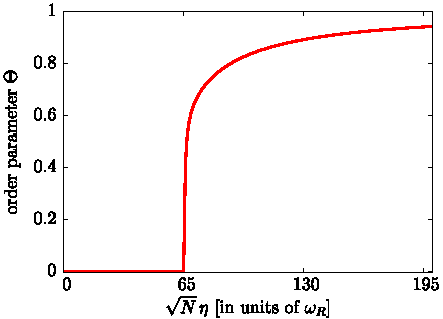
\includegraphics[width=1\linewidth]{images/order-parameter.pdf}
	\subcaption{Order parameter.}
	\end{minipage}
%
	\begin{minipage}[b]{.5\linewidth}
	\centering
	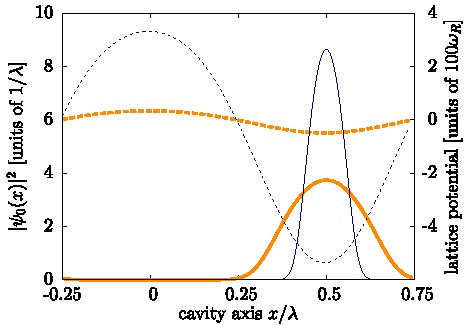
\includegraphics[width=1\linewidth]{images/lattice-potential.pdf}
	\subcaption{Lattice potential.}
	\end{minipage}
\caption{Order parameter and lattice potential for transversal pumping. Figures taken from~\cite{Nagy2008}.}
\label{fig:self-organization}
\end{figure}
\FloatBarrier